\fuxiti

\begin{xiaotis}

\xiaoti{计算:}
\begin{xiaoxiaotis}

    \begin{tblr}{columns={18em, colsep=0pt}}
        \xxt{$376 + 489$;} & \xxt{$742 - 145$;} \\
        \xxt{$64 \times 28$;} & \xxt{$893 \div 19$;} \\
        \xxt{$5487 + 694$;} & \xxt{$4503 - 784$;} \\
        \xxt{$325 \times 48$;} & \xxt{$4263 \div 87$;} \\
        \xxt{$8 + 7 \times 3$;} & \xxt{$18 - 10 \div 2$;} \\
        \xxt{$9 + 27 \div 3$;} & \xxt{$12 - 2 \times 5$;} \\
        \xxt{$36 \times 7 - 48 \div 2$;} & \xxt{$117 \div 13 + 64 \times 25$。} \\
    \end{tblr}

\end{xiaoxiaotis}


\xiaoti{计算:}
\begin{xiaoxiaotis}

    \begin{tblr}{columns={18em, colsep=0pt}}
        \xxt{$15.8 + 2.74$;} & \xxt{$4.2 - 0.39$;} \\
        \xxt{$3.5 \times 0.68$;} & \xxt{$12.96 \div 0.072$。} \\
    \end{tblr}

\end{xiaoxiaotis}


\xiaoti{计算:}
\begin{xiaoxiaotis}

    \begin{tblr}{columns={12em, colsep=0pt}, stretch=1.5}
        \xxt{$\dfrac{3}{5} + \dfrac{1}{5}$;} & \xxt{$\dfrac{5}{6} - \dfrac{1}{6}$;}  & \xxt{$\dfrac{1}{2} + \dfrac{2}{3}$;} \\
        \xxt{$\dfrac{2}{3} - \dfrac{1}{4}$;} & \xxt{$\dfrac{1}{6} + \dfrac{3}{10}$;} & \xxt{$3\dfrac{1}{4} - 2\dfrac{5}{6}$。} \\
    \end{tblr}

\end{xiaoxiaotis}


\xiaoti{计算:}
\begin{xiaoxiaotis}

    \begin{tblr}{columns={12em, colsep=0pt}, stretch=1.5}
        \xxt{$\dfrac{3}{5} \times \dfrac{1}{5}$;} & \xxt{$\dfrac{5}{6} \div \dfrac{1}{6}$;}    & \xxt{$\dfrac{7}{8} \times \dfrac{4}{5}$;} \\
        \xxt{$\dfrac{8}{9} \div \dfrac{5}{6}$;}   & \xxt{$1\dfrac{1}{2} \times \dfrac{1}{6}$;} & \xxt{$\dfrac{3}{4} \div 2\dfrac{1}{2}$。} \\
    \end{tblr}

\end{xiaoxiaotis}


\xiaoti{计算:}
\begin{xiaoxiaotis}

    \begin{tblr}{columns={18em, colsep=0pt}}
        \xxt{$31\% + 1.5\%$;}      & \xxt{$1 + 0.5\%$;} \\
        \xxt{$27\% - 12.4\%$;}     & \xxt{$1 - 35\%$;} \\
        \xxt{$32 \times 2.4\%$;}   & \xxt{$100 \times 0.1\%$;} \\
        \xxt{$1 \div 25\%$;}       & \xxt{$0.75 \div 15\%$。} \\
    \end{tblr}

\end{xiaoxiaotis}


\xiaoti{比较下列每对数的大小:}
\begin{xiaoxiaotis}

    \begin{tblr}{columns={18em, colsep=0pt}, stretch=1.5}
        \xxt{$\dfrac{4}{9}$ 和 $\dfrac{8}{9}$;}    & \xxt{$\dfrac{1}{10}$ 和 $\dfrac{1}{100}$;} \\
        \xxt{$\dfrac{7}{11}$ 和 $\dfrac{7}{22}$;}  & \xxt{$\dfrac{5}{7}$ 和 $\dfrac{7}{9}$;} \\
        \xxt{$0.78$ 和 $0.87$;}                    & \xxt{$\dfrac{3}{4}$ 和 $0.7$。} \\
    \end{tblr}

\end{xiaoxiaotis}


\begin{enhancedline}
\xiaoti{把有理数 $6.4$,$-9$,$\dfrac{2}{3}$,$+10$,$-\dfrac{3}{4}$,$-0.02$,$1$,$-1$,$7\dfrac{1}{3}$,$-8.5$,$25$,$-100$
    按正整数、负整数、正分数、负分数分成四个集合。
}

\xiaoti{有理数 $-3$、$+8$、$-\dfrac{1}{2}$、$+0.1$、$0$、$\dfrac{1}{3}$、$-10$、$-5$、$-0.4$ 中,
    哪些属于整数的集合,哪些属于分数的集合,哪些属于正数的集合,哪些属于负数的集合?
}

\xiaoti{把表示下列各数的点画在数轴上,再按从大到小的顺序,用“$>$” 号把这些数连结起来:
    $$ +3,\; -5,\; +5\dfrac{1}{2},\; -2\dfrac{1}{2},\; -4,\; +4,\; 0 \juhao $$
}

\xiaoti{按照从小到大的顺序,用“$<$” 号把下列各数连结起来:
    $$ -4\dfrac{1}{2},\; \dfrac{2}{3},\; 0.6,\; -0.6,\; -4.2,\; 5\juhao $$
}

\xiaoti{水冻结成冰的温度是 $0$ ℃,酒精冻结的温度是 $-117$℃,水银冻结的温度是 $-39$℃。
    哪一个冻结温度最高,哪一个最低?
}
\end{enhancedline}

\xiaoti{在数轴上画出大于 $-5$ 而小于 $+5$ 的所有整数。}

\xiaoti{在图中五个有理数组成的集合里找出最大数与最小数。}

\begin{figure}[htbp]
    \centering
    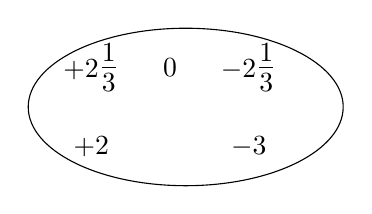
\begin{tikzpicture}
    \draw (2, 0) circle [x radius=2, y radius=1];

    \node at (0.8, 0.5) {$+2${\Large$\frac{1}{3}$}};
    \node at (1.8, 0.5) {$0$};
    \node at (2.8, 0.5) {$-2${\Large$\frac{1}{3}$}};
    \node at (0.8, -0.5) {$+2$};
    \node at (2.8, -0.5) {$-3$};
\end{tikzpicture}

    \caption*{(第 13 题)}
\end{figure}


\xiaoti{一个数的绝对值一定是正数吗? 为什么?}

\xiaoti{有理数中有没有最小的数? 有没有绝对值最小的数?
    有没有最小的正整数? 有没有最小的负整数? 如果有, 各是什么数?
}

\xiaoti{加工一根轴, 图纸上注明它的直径是 $\phi 30\,^{+0.03}_{-0.02}$,
    $\phi 30$ 表示直径是 30 毫米,
    $+0.03$ 表示合格品的直径最大只能比规定直径大 $0.03$ 毫米,
    $-0.02$ 表示合格品的直径最小只能比规定直径小 $0.02$ 毫米。
    那么合格品的直径最大是多少,最小是多少?
}

\begin{figure}[htbp]
    \centering
    \begin{tikzpicture}
    \pgfmathsetmacro{\angle}{45}
    \pgfmathsetmacro{\len}{5}
    \pgfmathsetmacro{\r}{1}

    \coordinate (O) at (0, 0);
    \coordinate (O') at ({\len * cos(\angle)},  {\len * sin(\angle)});
    \coordinate (dA) at ({\r * cos(90 + \angle)}, {\r * sin(90 + \angle)});
    \coordinate (dB) at ({\r * cos(270 + \angle)}, {\r * sin(270 + \angle)});

    \draw (O) circle (\r);
    \draw [pattern={mylines[angle=45, distance={4pt}]}]
        ($(O) + (dA)$) -- ($(O') + (dA)$)
        arc [start angle=90 + \angle, end angle=-90 + \angle, radius=\r]
        -- ($(O) + (dB)$)
        arc [start angle=-90 + \angle, end angle=90 + \angle, radius=\r];

    \draw (-1.5*\r, 0) -- (-\r, 0)
         (\r, 0) -- (1.5*\r, 0);
    \draw [dashed] (-\r, 0) -- (\r, 0);
    \draw (0, -1.5*\r) -- (0, -\r)
         (0, \r) -- (0, 1.5*\r);
    \draw [dashed] (0, -\r) -- (0, \r);

    \begin{scope}[xshift=15em, >=Stealth]
        \draw (0, 0) circle (\r);
        \draw (-1.5*\r, 0) -- (-\r, 0)
             (\r, 0) -- (1.5*\r, 0);
        \draw [dashed] (-\r, 0) -- (\r, 0);
        \draw (0, -1.5*\r) -- (0, -\r)
            (0, \r) -- (0, 1.5*\r);
        \draw [dashed] (0, -\r) -- (0, \r);

        \coordinate (X) at ({\r * cos(\angle)}, {\r * sin(\angle)});
        \coordinate (O) at (0, 0);
        \draw [<->] (X) -- ($(X)!2!(O)$);
        \draw (X) -- ($(X)!-1.5!(O)$) -- +(2, 0)
            node [pos=0.5, above] {$\phi 30\,^{+0.03}_{-0.02}$};
    \end{scope}
\end{tikzpicture}

    \caption*{(第 16 题)}
\end{figure}



\xiaoti{场上 30 袋稻谷过秤, 各袋的千克数记录如下:\\
    \begin{tblr}{columns={3em, $$}, colsep = 0pt, rowsep=0pt}
        93,  &   88,  &   91,  &   90,  &   89,  &   95,  &   86,  &   90,  &   90,  &   86,  \\
        94,  &   87,  &   85,  &   96,  &   94,  &   91,  &   95,  &   84,  &   87,  &   95,  \\
        90,  &   96,  &   89,  &   94,  &   88,  &   93,  &   92,  &   96,  &   90,  &   94\juhao
    \end{tblr} \\
    以每袋 90 千克为准, 超过的千克数记作正数, 不足的千克数记作负数,
    计算超过或不足的总数,并求 30 袋稻谷的总重量。
}


\xiaoti{第三中学男子排球队共有十名队员, 身高分别为:\\
    1.73 米, 1.74 米, 1.70 米, 1.76 米, 1.80 米, \\
    1.75 米, 1.77 米, 1.79 米, 1.74 米, 1.72 米。 \\
    计算男排队员平均身高。
}

\xiaoti{$9$ 与 $-13$ 的和是多少? 它们的和的绝对值是多少? 它们的绝对值的和是多少? 比较三个结果的大小。}

\xiaoti{写出下列各数的相反数和倒数:\jiange \\
    \begin{tblr}{hlines, vlines,
        columns={3em, c, $$},
        column{1} = {mode=text},
    }
        原数 & 5 & -6 & \dfrac{2}{3} & 1 & -0.5 & -1 \\
        相反数 & \\
        倒数 & \\
    \end{tblr} \jiange
}

\xiaoti{任意写出两个互为相反数的数。它们的和与商各是什么?}

\xiaoti{}%
\begin{xiaoxiaotis}%
    \xxt[\xxtsep]{两个有理数相乘, 在什么情况下积是正数? 是负数?是零?}

    \xxt{两个有理相除, 在什么情况下商是1 ? 是 $-1$ ? 是零?没有意义?}

\end{xiaoxiaotis}

\xiaoti{某冷冻厂 \, 一号 \, 库房的室温是 $-2$ ℃, 现有一批食品需要在 $-23$ ℃ 冷藏。
    如果每小时能降温 $4$℃,几小时后就能降到所要求的温度?
}

\xiaoti{煤矿 \, 井下 $A$ 点的标高是 $-174.8$ 米,己知从 $A$ 到 $B$,
    水平距离为 $120$ 米, 每经过水平距离 $10$ 米上升 $0.4$ 米, 求 $B$ 点的标高。
}

\begin{figure}[htbp]
    \centering
    \begin{tikzpicture}[>=Stealth, scale=0.85]
    \clip (0.05, 0) rectangle (7.95, -5.95);
    \draw (0, 0) -- (8, 0);
    \fill [pattern = dots] (0, 0) rectangle (8, -6);

    \filldraw [fill=white] (2, -4.2) -- (6, -3.0) --  (6, -3.8) -- (2, -5.0) -- cycle;

    \filldraw [fill=white] (1.5, 0) rectangle (2.3, -6);
    \filldraw [fill=white] (5.8, 0) rectangle (6.6, -6);

    \fill [fill=white] (2, -4.2) -- (6, -3.0) --  (6, -3.8) -- (2, -5.0) -- cycle;

    \node at (2.0, -4.8) {$A$};
    \node at (6.1, -3.8) {$B$};
    \draw [dashed] (2.3, -4.95) -- (5.8, -4.95)
        node [pos=0.6, below, fill=white, inner sep=3pt] {$120$};
\end{tikzpicture}

    \caption*{(第 24 题)}
\end{figure}


\xiaoti{计算:}
\begin{xiaoxiaotis}

    \begin{tblr}{columns={18em, colsep=0pt}}
        \xxt{$5 \div 0.1$;}        & \xxt{$5 \div 0.01$;} \\
        \xxt{$5 \div 0.001$;}      & \xxt{$5 \div (-0.1)$;} \\
        \xxt{$5 \div (-0.01)$;}    & \xxt{$5 \div (-0.001)$;} \\
        \xxt{$0.2 \div 0.1$;}      & \xxt{$0.02 \div 0.01$;} \\
        \xxt{$0.002 \div 0.001$;}  & \xxt{$(-0.3) \div 0.1$;} \\
        \xxt{$(-0.03) \div 0.01$;} & \xxt{$(-0.003) \div 0.001$。} \\
    \end{tblr}

\end{xiaoxiaotis}


\xiaoti{在下列各式的括号里填上适当的数:}
\begin{xiaoxiaotis}

    \xxt{\begin{tblr}[t]{columns={$}}
        (+5) + (\quad) = +3, \\
        (+5) + (\quad) = -3, \\
        (-5) + (\quad) = +3, \\
        (-5) + (\quad) = -3; \\
    \end{tblr}}

    \xxt{\begin{tblr}[t]{columns={$}}
        (+3) \times (\quad) = -6, \\
        (-3) \times (\quad) = -6, \\
        (+6) \times (\quad) = +3, \\
        (+6) \times (\quad) = -3; \\
    \end{tblr}}

    \xxt{\begin{tblr}[t]{columns={$}}
        (-3) + (\quad) = 0, \\
        (-5) \times (\quad) = 0\juhao \\
    \end{tblr}}

\end{xiaoxiaotis}


\xiaoti{在下面各式的括号里,能不能填上适当的数?}
\begin{xiaoxiaotis}

    \twoInLineXxt[18em]{$0 \times (\quad) = 5$;}{$0 \times (\quad) = 0$。}

\end{xiaoxiaotis}


\xiaoti{平方得 $4$ 的有理数有哪几个? 有没有平方得 $-4$ 的有理数?
        立方得 $8$ 的有理数有哪几个? 有没有立方得 $-8$ 的有理数?
}


\begin{enhancedline}
\xiaoti{计算}
\begin{xiaoxiaotis}

    \xxt{$\left(1\dfrac{3}{4} - \dfrac{7}{8} - \dfrac{7}{12}\right) \times \left(-1\dfrac{1}{7}\right)$;}

    \xxt{$(-81) \div 2\dfrac{1}{4} + \dfrac{4}{9} \div (-16)$;}

    \xxt{$\dfrac{2}{5} \div \left(-2\dfrac{2}{5}\right) - \dfrac{8}{21} \times \left(-1\dfrac{3}{4}\right) - 0.25$;}

    \xxt{$3 (-2.5) (-4) + 5 (-6) (-3)^2$;}

    \xxt{$\{0.85 - [12 + 4 \times (3 - 10)]\} \div 5$;}

    \xxt{$2^2 + (-2)^3 \times 5 - (-0.28) \div (-2)^2$;}

    \xxt{$[(-3)^3 - (-5)^3] \div [(-3) - (-5)]$。}

\end{xiaoxiaotis}
\end{enhancedline}

\xiaoti{按下列程序进行计算,并把各次结果填入表内(如第一次 $(+3) \times (+3) - (-5)$ 得 $14$,不大于 $200$;
    第二次再做,$14 \times (+3) - (-5)$,等等):
}

\begin{minipage}{7cm}
    \centering
    \begin{tikzpicture}[
    >=Stealth,
    skip loop/.style={to path={-- ++(#1, 0) |- (\tikztotarget)}},
]
    \graph [grow down sep = 2em,
        nodes={draw, rectangle, minimum width=7em},
        decision/.style={draw, diamond, aspect=4, inner sep=1pt},
    ]{
        add/"$+3$" [label=above:{输入}] ->
        times/"$\times (+3)$" ->
        sub/"$- (-5)$" ->
        decide/"$>200$" [decision, label=3:{否}] ->["是"]
        stop/"停" [label=below:{输出}];
    };

    \graph[no placement] {
        p1 [coordinate, below=3mm of add];
        (decide.east) -> [skip loop=10mm] (p1);
    };
\end{tikzpicture}

\end{minipage}
\begin{minipage}{7cm}
    \begin{tblr}{hlines, vlines,
        colspec={Q[c,6em]Q[c,6em]},
    }
        计算次数 & 计算结果 \\
        1       & 14       \\
        2       &          \\
        3       &          \\
        4       &          \\
    \end{tblr}
\end{minipage}



\xiaoti{按下列程序进行计算,并把各次结果填入表内:}

\begin{minipage}{7cm}
    \centering
    \begin{tikzpicture}[
    >=Stealth,
    skip loop/.style={to path={-- ++(#1, 0) |- (\tikztotarget)}},
]
    \graph [grow down sep = 2em,
        nodes={draw, rectangle, minimum width=7em},
        decision/.style={draw, diamond, aspect=4, inner sep=1pt},
    ]{
        sub/"$-2$" [label=above:{输入}] ->
        add/"$+ (-1.5)$" ->
        div/"$\div (+2)$" ->
        decide/"$> -1.6$" [decision, label=3:{否}] ->["是"]
        stop/"停" [label=below:{输出}];
    };

    \graph[no placement] {
        p1 [coordinate, below=3mm of sub];
        (decide.east) -> [skip loop=10mm] (p1);
    };
\end{tikzpicture}

\end{minipage}
\begin{minipage}{7cm}
    \begin{tblr}{hlines, vlines,
        colspec={Q[c,6em]Q[c,6em]},
    }
        计算次数 & 计算结果 \\
        1       &          \\
        2       &          \\
        3       &          \\
    \end{tblr}
\end{minipage}

\end{xiaotis}

